\documentclass[./main.tex]{subfiles}

\begin{document}
\chapter*{why this effort?}

Well I think about a lot of things (with some rigor) and it seems that after a point I am not able to keep track of them.
I forget some important conclusions, perspectives, schools of thought, jewels of wisdom and such things in various aspects that are fruits of a lot of effort, suffering and pain.
And I often have to re-start my train of thought on them, which is tedious and dis-motivating after a point of time.

\paragraph{Therefore this journal is to}

\begin{enumerate}
  \item Write down stuff
    \begin{enumerate}
      \item So that I don't lose it permanently.
      \item So that I don't have to remember what I don't need to.
      \item In a condensed, simplified, clean, elegant, minimalistic form.
      \item So that I use my brain for thinking rather than storing.
    \end{enumerate}
  \item Use the power of search.
  \item Don't start over from scratch. Build on previous knowledge.
\end{enumerate}

\begin{figure}[h]
  \centering
  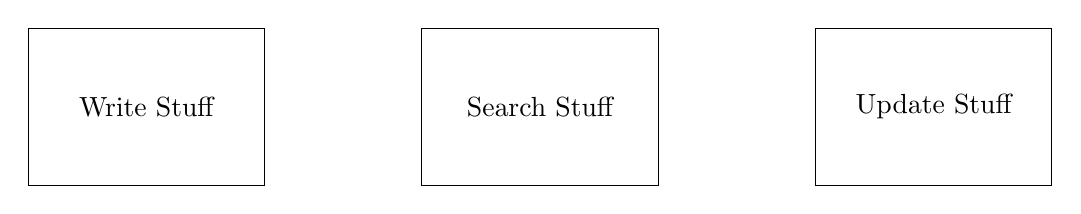
\begin{tikzpicture}
    \draw (0, 0) rectangle (3, 2) node[pos=0.5] {Write Stuff};
    \draw (5, 0) rectangle (8, 2) node[pos=0.5] {Search Stuff};
    \draw (10, 0) rectangle (13, 2) node[pos=0.5] {Update Stuff};
  \end{tikzpicture}
\end{figure}

\paragraph{The effort will be to}
\begin{enumerate}
  \item Forget everything I think I know.
  \item Keep everything as simple and minimalistic as possible.
  \item Build constructs that are simple, atomic, composable and do one thing excellently.
  \item Have a minimal number of (and thus obviously finite) constructs.
  \item Build connections and flow among the instances of constructs.
  \item Promote recognition rather than re-call.
\end{enumerate}
These ideas are inspired by the UNIX philosophy, my experience in programming and doing things in general.

\end{document}
